\documentclass[twocolumn]{jbook}
\usepackage[dvipdfmx]{graphicx}
\usepackage{bm,braket,ascmac,extarrows}
\usepackage{amsmath,amssymb,amsthm,mathrsfs,makeidx}
\usepackage{amsfonts,graphics,fancyhdr,ulem,stmaryrd}
\usepackage[all]{xy}
\usepackage[%
top    = 15truemm,%
bottom = 15truemm,%
left   = 6truemm,%
right  = 6truemm]{geometry}
\usepackage{amsthm, bm}

\usepackage{tikz}
\usetikzlibrary{shadows}
\usetikzlibrary{patterns}

\pagestyle{fancy}
\lhead{\rightmark}
% Theorem 環境
\theoremstyle{definition}


%メモでつかう%
\newtheorem{theo}{定理}
\newtheorem{lem}[theo]{補題}
\newtheorem{prop}[theo]{命題}
\newtheorem{prob}[theo]{問題}
\newtheorem{example}[theo]{例}
 
%Enumerate 環境
\def\theenumi{\arabic{enumi}}
\def\labelenumi{(\theenumi)}

% (Re)New commands


\newcommand{\abs}[1]{\left|#1\right|}

\newcommand{\bolm}[1]{{\mbox{\boldmath $#1$}}}
\newcommand{\tf}[1]{\textbf{#1}}
\newcommand{\maru}{\textcircled}
\newcommand{\symdiff}{\bigtriangleup}
\newcommand{\ovl}{\overline}
\newcommand{\lan}{\langle}
\newcommand{\ran}{\rangle}
\newcommand*{\vvv}{\overrightarrow}
\newcommand{\vin}{\rotatebox{90}{$\in$}}
\newcommand{\thm}{\begin{itembox}[l]}
\newcommand{\jap}{\mbox}
\newcommand{\enthm}{\end{itembox}\\}
\newcommand{\disp}{\displaystyle}
\newcommand{\dou}{\Leftrightarrow}
\newcommand{\del}{\partial}
\newcommand{\ben}{\begin{enumerate}}
\newcommand{\een}{\end{enumerate}}
\newcommand{\beqn}{\begin{eqnarray*}}
\newcommand{\eeqn}{\end{eqnarray*}}
\newcommand{\bcas}{\begin{cases}}
\newcommand{\ecas}{\end{cases}}
\newcommand{\nara}{\Rightarrow}
\newcommand{\mb}{\mathbb}
\newcommand{\mr}{\mathrm}
\newcommand{\maf}{\mathfrak}
\newcommand{\masc}{\mathscr}
\newcommand{\hana}{\mathcal} %花文字(花文字じゃない)
\newcommand{\chat}{\widehat{\mathbb{C}}} %リーマン球面
\newcommand{\khat}{\widehat{K}} %%Lemma4.5.6
\renewcommand{\leq}{\leqq}
\renewcommand{\geq}{\geqq}
\renewcommand\thefootnote{*\arabic{footnote}}
\newcommand{\nea}{\nearrow}
\newcommand{\exer}{{\bf 演習}\arabic{chapter}.\arabic{section}.}
\newcommand{\sea}{\searrow}
\newcommand{\witi}{\widetilde} %%%ワイドチルダ
\newcommand{\tens}{\mathbin{\otimes}}
\newcommand{\bracket}[1]{%
\[
 \left(
 \begin{tabular}{p{0.9\hsize}}
  #1
 \end{tabular}
 \right)
\]}

\newcommand{\step}[2]{{\large \textbf{Step.#1}}(#2)}

\newcommand{\parena}[1]{\left( #1\right)}
\newcommand{\parenb}[1]{\left\{ #1\right\}}
\newcommand{\parenc}[1]{\left[ #1 \right]}

\makeatletter
\def\mapstofill@{%
   \arrowfill@{\mapstochar\relbar}\relbar\rightarrow}
\newcommand*\xmapsto[2][]{%
   \ext@arrow 0395\mapstofill@{#1}{#2}}
\newcommand{\xequal}[2][]{\ext@arrow 0055{\equalfill@}{#1}{#2}}
\def\equalfill@{\arrowfill@\Relbar\Relbar\Relbar}
\makeatother

\begin{document}
\section*{11/14更新}
\section*{Q.046}
\textbf{Step 1.} $a^2\leq a$のとき。\\
このとき$0\leq a\leq 1$である。$x$が$(x-a)(x-a^2)<0$を満たすことと, 区間$(a^2,a)$に属することは同値である。しかし, $a$の範囲から$(a^2,a)\subset (0,1)$なので, 5つの整数を含めることは出来ない。よってこの場合解なし。

\textbf{Step 2.} $a^2>a$のとき。\\
$a<0$または$a>1$である。$x$は区間$(a,a^2)$に属する。この区間に整数が$5$個入っていれば良い。つまり, ある整数$N$が存在して
\[N\leq a < N+1<N+2<N+3<N+4<N+5<a^2\leq N+6\]
であればよいが, 整数$N$が$N\leq a<N+1$を満たすことは$N=\lfloor a\rfloor$であること, それと同様に$N+5<a^2\leq N+6$は$N+6=\lceil a^2 \rceil$と同じであることに注意すると, 
\[\lfloor a\rfloor + 6 = \lceil a^2\rceil\]
を$a$が満たすことと, $(a,a^2)$が整数を$5$個含むことは同値である。そこで, 上を満たす$a$を求めることとしよう。\par
$\lfloor x\rfloor$ $\lceil x^2 \rceil \geq x^2 $を使うと,
\[a + 6\geq a^2\quad \dou \quad (a-3)(a+2)\]
を満たすことが必要条件となる。よって$-2\leq a\leq 3$が必要条件である。以下, $\lfloor a\rfloor=k$の値で場合分け($k=-2,-1,0,1,2,3$)をする。
\ben
\item[(i)] $k=-2$のとき\\
$-2\leq a<-1$かつ, $4=\lceil a^2\rceil$となる。
\[\lceil a^2\rceil =4 \dou 3< a^2 \leq 4\]
であるから, $-2\leq a < -\sqrt{3}$である。
\item[(ii)] $k=-1$のとき\\
$-1\leq a<0$かつ,
\[\lceil a^2\rceil = 5 \dou 4< a^2\leq 5\]
なので解なし。
\item[(iii)] $k=0$のとき\\
$0\leq a<1$かつ$5<a^2\leq 6$なので解なし。
\item[(iv)] $k=1$のとき\\
$1\leq a<2$かつ$6<a^2\leq 7$なので解なし。\\
\item[(v)] $k=2$のとき\\
$2\leq a<3$かつ$7<a^2\leq 8$である。これは$\sqrt{7} < a < 2\sqrt{2}$のときである。
\item[(vi)] $k=3$のとき\\
$-2\leq a\leq 3$かつ$k=3$なので$a=3$のときである。これは$\lceil 9 \rceil = 9$を満たすので解である。
\een
以上より
\[\bolm{ -2\leq a<-\sqrt{3},\quad \sqrt{7}<a<2\sqrt{2},\quad a=3 }\]

\section*{Q.065}
\ben
\item $X=5\cdot 2^{7}$とする。注意より$X+1=641$であるが, 
\beqn
5^{4}\cdot 2^{28} + 2^{32} &=& 2^{28}(5^4+2^4)=2^{28}\cdot 641\\
5^{4}\cdot 2^{28}-1 &=& X^4-1 \\
&=& (X+1)(X-1)(X^2+1)\\
&=&641(X-1)(X^2+1)
\eeqn
となるので, いずれも641の倍数である。\qed
\item $(5^4\cdot 2^{28}+2^{32}) - (5^4\cdot 2^{28} -1) = 2^{32}+1$で, 左辺が641の倍数同士の和なのでこれも641の倍数である。
\een

\section*{Q.090}
\ben
\item $n$の10進法表示は
\[n=\disp\sum_{k=0}^{N}a_k10^{k} \quad (N\geq 0, a_k\in \{0,1,\cdots, 9 \}\]
であるが, これの$\bmod{9}$が
\[n\equiv \disp\sum_{k=0}^{N}a_k(10-9)^{k} = \disp\sum_{k=0}^{N} a_k \pmod{9}\]
となり, 右辺はまさしく桁の数字の総和を表す。\qed
\item 入っていない桁を$a$とする。$a$は$\{ 0,1,\cdots, 9\}$の元である。このとき, $2^{29}$の桁の総和は
\[0+1+2+\cdots + 8+9 - a= 45-a\]
である。一方で, $2^{29}\equiv 5 \pmod{9}$であるから, $5\equiv 45-a$でなければならない。これを解くと$a\equiv 4\pmod{9}$となり,$a$は$\{ 0,1,\cdots, 9\}$の元であるから, $a=4$である。
\een

\clearpage


\section*{Q.74}
\ben
\item $u=1+\sqrt{2}$であることを示す。$G\ni u>1$はよい。$1<w\leq u$なる$w\in G$を考え, $w=a+b\sqrt{2}$とおく。$|a^2-2b^2| = w|a-b\sqrt{2}|=1$であるから, 
\[|a-b\sqrt{2}| = \dfrac{1}{w} < 1 \quad (\because w>1)\]
より, $-1<a-b\sqrt{2} < 1$となる。これと$1<w=a+b\sqrt{2}$が成り立つから, 
\[-1+1 < (a-b\sqrt{2}) + (a+b\sqrt{2}) \]
\[1+(a-b\sqrt{2}) < 1 + (a+b\sqrt{2})\]
が成り立つ。整理して$0<a$, $0<b$を得るので, $1\leq a, 1\leq b$でなければならず, 結局
\[1+\sqrt{2} = u \leq w\]
となる。$1<w\leq u$としたから, $w=u$となる。すなわち$u$は最小である。
\item 次を示す。
\beqn
w_1, w_2\in G&\nara& w_1w_2\in G
\eeqn
$w_i=a_i+b_i\sqrt{2}$\quad ($a_i^2 - 2b_i^2 = \pm 1$, $w_i>0$) とおく。$w_1w_2 > 0$であることは明らか。積を計算すると
\beqn
w_1w_2 = (a_1a_2 + 2b_1b_2) + \sqrt{2}(a_2b_1 + a_1b_2)
\eeqn
であるが, 
\beqn
&&(a_1a_2 + 2b_1b_2) ^2 - 2(a_2b_1 + a_1b_2)^2\\
&=& (a_1a_2)^2 + 4(b_1b_2)^2 - 2(a_2b_1)^2 - 2(a_1b_2)^2\\
&=&(a_1^2 - 2b_1^2)(a_2^2-2b_2^2)\\
&=&\pm 1 \quad (a_i^2-2b_i^2 \in \{ -1,1 \})
\eeqn
となる。よって, $w_1w_2\in G$が示された。つまり「$G$は積で閉じている」ことが示された。\par
次に整数$n$に対して$u^{n}\in G$を示す。$n=0$のときは$u^{0}=1$で, 明らかに$G$に含まれる。
$n$が正なら, $u\in G$から, 先の積で閉じていることを用いると$u^{n}\in G$となる。$n$が負なら, $(u^{-1})^{-n}$を考え, $u^{-1} = \sqrt{2} -1 \in G$なので, この場合も$G$が積で閉じていることから, $u^n$は$G$に属する。よって, すべての$n \in \mb{Z}$で$u^n\in G$である。\par
最後に, $w_1=g$, $w_2=u^n$として適用すれば$gu^n\in G$が導かれ, 題意は示された。\qed
\item $G$の元$g$をひとつ取る。このとき, ある整数$n(g)$が存在して
\[u^{n(g)-1} < g \leq u^{n(g)}\]
を満たす。両辺を$u^{n(g)-1}$で割ると
\[1 < gu^{-n(g)+1} \leq u\]
であり, (2)で示したことから$gu^{-n(g)+1}$は$G$の元であって, さらに1より大きい。(1)で$u$の最小性を示したので, $gu^{-n(g)+1} = u$でなければならない。よって$g=u^{n(g)}$を得るから, 題意は示された。\qed


\een



\subsection*{Q.162(12/2更新)}
体積を求める領域を$K$とし, その体積を$V$とする。曲線$y=\log{x}$ ($1\leq x \leq e$) を$x$軸で回転させたときの曲面は
\[\bcas
y^2+z^2 = (\log{x})^2\\
1\leq x\leq e
\ecas\]
として表せる。この曲面は$xz$平面対称であるから$K$もそうであり, $K$のうちの$y\geq 0$の部分の体積は$\dfrac{1}{2}V$である。\par
$K$は$-1\leq y\leq 1$の範囲に存在するので, $y=k$ ($0\leq k\leq 1$) で$K$を切断したときの断面積を考える。上の$y$軸で回す前の曲面の定式化から, その曲面を$y=k$で切断した部分を$xz$平面へ射影すると
\[
\bcas
z^2 = (\log{x})^2 - k^2\\
e^{k} \leq x\leq e 
\ecas
\]
という曲線になるので, これを$C_k$と呼ぶこととする。$C_k$上の点$\mr{P}$は$(t,\pm\sqrt{(\log{t})^2 - k^2})$ と書くことができ($e^{k} \leq t\leq e$), 符号がいずれであっても$(0,0)$との距離は$t^2+(\log{t}^2) - k^2=:D(t)$となる。$D(t)$は明らかに$[e^{k}, e]$上増加するから, $ e^{2k} \leq D(t) \leq e^2+1-k^2$であることが分かる。これは, $C_k$上で最も原点に近い点が$(e^{2k}, 0)$であり, 最も遠い点が$(e,\sqrt{1-k^2})$であることから来る。よって, $C_k$を原点中心に回転させると, 極座標で表現して\bolm{円環領域 e^{k} \leq r \leq \sqrt{e^2+1-k^2}}になることが分かるので, これが$K$の平面$y=k$による断面である。つまり, その断面積を$S(k)$とおけば
\[S(k) = \pi(e^2+1-k^2 - e^{2k})\]
となる。よって, 
\beqn
\dfrac{1}{2}V &=& \disp\int_{0}^{1} S(y) \, dy \\
&=& \pi\disp\int_{0}^{1}(e^2+1-y^2 - e^{2y})\, dy\\
&=& (e^2+1)\pi - \pi\disp\int_{0}^{1} (y^2 + e^{2y})\, dy\\
&=& (e^2+1)\pi - \pi\left[ \dfrac{y^3}{3} + \dfrac{1}{2} e^{2y} \right]_{0}^{1}\\
&=& (e^2+1)\pi - \left\{\left(\dfrac{1}{3} - 0\right)\pi - \dfrac{1}{2}\left(e^2 - 1\right)\pi\right\}\\
&=& \left( \dfrac{1}{2}e^2 + \dfrac{7}{6} \right)\pi
\eeqn
以上より, \bolm{V=\left(e^2+\dfrac{7}{3}\right)\pi}




\clearpage






\subsection*{Q.126(12/3更新)}
まず, $\dfrac{d}{dx}(864n^2f(x)) = 3x(36n - x)$であることに注意すると, $f(x)$は区間$[0,36n]$上増加しているため, $i$を$0\leq i <36n$を満たす整数であるとして, $[f(i)] \leq [f(i+1)]$が常に成り立つことが分かる。したがって, このような$i$のうち, この不等式の等号を生じさせないものが$k$種類あるとすれば, 求める個数は$k+1$である。\par
$f(i+1) - f(i)-1$を計算してみる。
\beqn
&&\dfrac{1}{864n^2}\left\{ 54n((i+1)^2 - i^2)  - ((i+1)^3 - i^3)\right\}-1\\
&=& \dfrac{1}{864n^2}\left\{ -3i^2 + (108n -3)i + (54n-1)-864n^2 \right\}
\eeqn
$\{\quad \}$の中身の$i$の二次式について, 判別式$D$を計算する:
\[D=(108n-3)^2 +12(-864n^2 + 54n-1) =1296n^2 - 3\]
よって, 2次方程式$-3X^2 + (108n-3)X + (-864n^2 + 54n -1) = 0$の解は$X=18n-\dfrac{1}{2} \pm \dfrac{\sqrt{D}}{6}$と求まるので,
\beqn
f(i+1) - f(i) -1 \geq 0 \dou 18n-\dfrac{1}{2} -\dfrac{\sqrt{D}}{6} \leq i \leq 18n-\dfrac{1}{2} +\dfrac{\sqrt{D}}{6}
\eeqn
であることが分かる。$i$は整数で考えているが, それでもこの不等式を満たす整数というのは精密に考えることが出来る。つまり, 右の範囲を満たす$i$とは, $i$が整数であることを考慮すれば, 天井関数と床関数により
\[\left\lceil 18n-\dfrac{1}{2} -\dfrac{\sqrt{D}}{6}\right\rceil \leq i \leq \left\lfloor 18n-\dfrac{1}{2} + \dfrac{\sqrt{D}}{6} \right\rfloor\]
を満たす整数$i$ということができるが, この最左辺と最右辺については, $6n-\dfrac{1}{2} <  \dfrac{\sqrt{D}}{6} = \sqrt{36n^2 - \dfrac{1}{12}} < 6n$に注意すれば
\beqn
\left\lceil 18n-\dfrac{1}{2} -\dfrac{\sqrt{D}}{6}\right\rceil &=& 12n\\
\left\lfloor 18n-\dfrac{1}{2} + \dfrac{\sqrt{D}}{6} \right\rfloor&=& 24n-1
\eeqn
が従うので, 結局
\[f(i+1) - f(i) -1\geq 0 \dou 12n \leq i < 24n\]
となる。
つまり, この$i$の範囲においては $f(i) + 1 \leq f(i+1) \nara \left[ f(i)\right] < \left[ f(i+1) \right]$が成り立つ。これは, 
\[ 7n=[f(12n)] < [f(12n+1)] < \cdots < [f(24n)]=20n\]
という増加列$\{ [f(i)] \}$が, どの2つも違う整数を登場させるので, この部分には$7n$から$20n$の間に飛び飛びで$12n+1$個の整数が登場していることが分かる。
\par
逆に, $0\leq i<12n$あるいは$24n\leq i <36n$の場合は$f(i) \leq f(i+1) < f(i) +1$となるので, $[f(i)] \leq [f(i+1)]$の等号は成り立つ場合も成り立たない場合もあるけれども, 等号が成り立たない場合であるとしても, \bolm{ [f(i)] と [f(i+1)] の差は1にしかならない。}つまり, 
\[0=[f(0)] \leq [f(1)] \leq \cdots \leq [f(12n)] = 7n\]
という整数の広義増加列は, $0$から$6n$までの$7n+1$個の整数がスキップされることなく登場している。同様にして
\[20n=[f(24n)] \leq [f(24n+1)] \leq\cdots \leq [f(36n)] = 27n\]
の間の$7n+1$個の整数もすべて登場する。\par
以上のことから, 単に$(12n+1) + (7n+1) + (7n+1)$とすると, これは$7n$と$20n$を2つずつカウントすることになるので, 求める個数はそこから2を引いた
\[ \bolm{26n+1} \]
である。
\clearpage
\section*{1/20更新}

\ben
\item 二項定理を使う。以下の合同式は$\bmod{100}$である。
\[(10+1)^{11} = \disp\sum_{k=0}^{11} 10^{k} {}_{11}\mr{C}_{k}  \equiv 10\cdot {}_{11}\mr{C}_{1} + 1 \equiv \bolm{11}\]
\item 次の因数分解を利用する。
\beqn
&&3^{2^{n}} - 1 \\
&=& (3^{2^{n-1}}+1) (3^{2^{n-2}}+1) \cdots (3^{2^{1}} +1) (3^{2^{0}}+1)(3^{2^{0}} - 1)
\eeqn
ここで, $3^{2^{k}} + 1$ ($k=1,2,\cdots, n-1$) は$3^{2^{k}} + 1 \equiv 2\pmod{4}$によって$2$で$1$回しか割れない。また, $3^{2^0} + 1 = 4$, $3^{2^{0}} - 1 = 2$に注意すると, 上の式から$3^{2^{n}} -1$は$2$で$n+2$回割れる。よって$3^{2^{n}}  - 1 \equiv 0\pmod{2^{n+2}}$である。よって, 
\[3^{2^{n}}\equiv \bolm{1} \pmod{2^{n+2}}\]
となる。(数学的帰納法を使って証明する方法もある。)
\item $4444\equiv -2 \pmod{9}$により$(-2)^{4444}\bmod{9}$を見ればよい。$(-2)^{6} \equiv 64\equiv 1 \pmod{9}$なので
\beqn
(-2)^{4444} &\equiv& (-2)^{6\times 740 + 4} = 64^{740}\cdot (-2)^{4}\\
&\equiv& 1^{640}\cdot 16 \equiv \bolm{7} \pmod{9}
\eeqn
\item $\disp\prod_{k=1}^{999}(10^{k}-1)$という数である($\disp\prod$は総積の記号)。よって, 
\beqn
\disp\prod_{k=1}^{999} (10^{k} - 1) &=& 9\times 99\times \disp\prod_{k=1}^{997} (10^{k+2} - 1)\\
&\equiv& 891\disp\prod_{k=1}^{997} (-1)\\
&=&891(-1)^{997}\\
&\equiv& \bolm{109}
\eeqn
\item この場合, $\bmod{100}$を考えるよりは$\bmod{4}$と$\bmod{25}$に分けてそれぞれを調べるとよい。これは, $100$を互いに素な$2$つの数の積$4\times 25$と考えて$\bmod{4}$, $\bmod{25}$を調べれば, $\bmod{100}$の値が復元できるということ(中国剰余定理)を利用している。\\
$6^{2017} \equiv 0\pmod{4}$である。よって, $6^{2017} = 4k_1$ ($k_1\in \mb{Z}$)と書ける。\par
二項定理より
\beqn
6^{2017} = (5+1)^{2017} \equiv {}_{2017}\mr{C}_{1} \cdot 5 + 1 \equiv 11\pmod{25} 
\eeqn
なので, $6^{2017}=25k_2 + 11$ ($k_2\in \mb{Z}$)と書ける。いま, $4k_1 = 25k_2 + 11$が成り立っているが, $\bmod{4}$を取ると$k_2\equiv 1 \pmod{4}$が従う。よって, $k_2 =4k_3+1$ ($k_3\in \mb{Z}$)と書くことができる。したがって, 
\[6^{2017} = 25k_2+11 = 25(4k_3  + 1) + 11 = 100k_3 + 36\]
となるので, $\bmod{100}$の値が復元でき, $6^{2017}\equiv 36\pmod{100}$となる。
\item $10$の$\pmod{13}$による位数を考える。つまり, $10^{d} \equiv 1\pmod{13}$となるような最小の自然数$d$を求める。一般に剰余類の数$a$とmodを取る数$b$が互いに素ならそのような位数は存在し, その位数は「$\phi(b)$の約数」の中で取れる。この場合なら, $\phi(13)=12$なので$12$の約数から見てあげるとよい。\par
実際, $10^{6} \equiv (-3)^{6} \equiv (-27)^{2} \equiv (-1)^{2} \equiv 1 \pmod{13}$である。大切なのは, そのように$6$が位数とわかったとき, $10^{m}$を$6$で割ることを考えて$10^{m} = 6k + r$ ($k\in\mb{Z}, 0\leq r<6$) と表したとき, 
\[10^{10^{m}} = 10^{6k} \cdot 10^{r} \equiv (10^{6})^{k} \cdot 10^{r} \cdot 1^{k} \cdot 10^{r} \equiv 10^{r}\pmod{13}\]
となることである。そこで, $r$, つまり$10^{m}\bmod{6}$を求めればよいことになる。調べればわかるように, $10^{m} \equiv 4\pmod{6}$がすべての自然数$m$で成り立つので$r=4$としてとれる。よって, 
\[10^{10^{m}} \equiv 10^{4} \equiv (-3)^{4} = 81 \equiv \bolm{3}\pmod{13}\]
\item 階乗のある素因数の指数を決定する方法はルジャンドルの定理による。この場合, $2017!$に$5$が何回かけられているかは, 
\beqn
\lfloor \dfrac{2014}{5}\rfloor = 402, \lfloor \dfrac{2014}{25}\rfloor = 80, \lfloor \dfrac{2014}{125}\rfloor = 16,\\
\lfloor \dfrac{2014}{625}\rfloor = 3,  \lfloor \dfrac{2014}{5^{k}}\rfloor = 0\, (\mr{for} \, k\geq 5)
\eeqn
に出てきたすべての数を足し合わせればよい。つまり, $402+80+16+3= 501$であり, $2014! = 5^{501}m$ のように書ける。$m=25k+r$ ($0\leq r<25$)と書いたとき, $2014! =5^{503}k + 5^{501}r$となるので, $r$が分かると$2014!\bmod{5^{503}}$もわかる。$r$は$\dfrac{2014!}{5^{501}}$の$25$で割ったあまりとして求まるので, この$\dfrac{2014!}{5^{501}}$を調べたい。\par
$f(n) = (5n+1)(5n+2)(5n+3)(5n+4)$とする。まず, すべての$n$に対して
\[f(n) \equiv -1 \pmod{25}\]
であることに注意せよ。これは展開からただちに従う。\par
方針としては, $i=0,1,2,3$に対して, $2014!$の中から「$5^{i}$の倍数だが$5^{i+1}$の倍数でないもの」だけを取り出した積$P_i$を調べることである。それらを, $f(n)$を利用して表現する。\\
まず$P_0$は次のようになる。
\[P_0 = f(0)f(1) \cdots  f(402)\], 
$P_1$は, $2005,2010$が微妙に余るが, 次のように書ける。
\[P_1 = (5^4f(0))(5^4f(1))\cdots (5^4f(79))\times  2005 \times 2010\]
同様に, 
\beqn
P_2= (25^4f(0)) (25^{4}f(1))\cdots (25^4f(15))\\
P_3= (125^4f(0))(125^4f(1))(125^4f(2)) \times 2000\\
P_4= 625^3(1\times 2\times 3)
\eeqn
したがって, $2014! = P_0P_1P_2P_3P_4$である。$\dfrac{2014!}{5^{501}}$は, $P_i$から$5$の部分を消せばよい。きりの悪い部分をかき集めて$C=2005\times 2010\times 2000 \times P_4$とし, $5$の成分のみ取り出して$C=5^{17}D$とする($D$は$5$で割れない整数である)。いま, 
\beqn
2014! = C\disp\prod_{k=0}^{402}f(k) \disp\prod_{l=0}^{79}5^{4}f(l) \disp\prod_{m=0}^{15}25^{4}f(m) \disp\prod_{n=0}^{2} 125^{4}f(n)
\eeqn
であるから, $5^{501}$で割ると, $5$の成分は消失して
\beqn
\dfrac{2014!}{5^{501}} &=& D\disp\prod_{k=0}^{402}f(k) \disp\prod_{l=0}^{79}f(l) \disp\prod_{m=0}^{15}f(m) \disp\prod_{n=0}^{2} f(n)\\
&\equiv & D(-1)^{403}(-1)^{80}(-1)^{16}(-1)^{3} \quad (\because f(n)\bmod{25} = 1)\\
&\equiv& D \pmod{25}
\eeqn
となる。$D=401\times 402\times 16 (1\times 2\times 3)$であったから, 
\beqn
D\equiv 1\times 2\times 16\times 1\times 2\times 3 \equiv 17\pmod{25}
\eeqn
より, $r=17$としてとれるから, 
\[\bolm{ 2014! \equiv 17\cdot 5^{501} \pmod{5^{503}}}\]

\item 問題文に不備がある。本問では$p\geq 3$である。\\
${}_{p-1}{\mr{C}}_{\frac{p-1}{2}} \equiv k \pmod{p}$とする。以下のmoduloは$\bmod{p}$とする。このとき, 左辺の階乗を払うことで
\[(p-1)! \equiv k\left( \dfrac{p-1}{2} ! \right)^2\]
となる。ここで, 右辺の$\left(\dfrac{p-1}{2}\right)^2$は片方の$\left(\dfrac{p-1}{2}\right)!$を
\[\left(\dfrac{p-1}{2}\right)! \equiv \left(-\dfrac{p+1}{2}\right) \cdot\left(- \dfrac{p+3}{2}\right)\cdot \cdots \cdot \left\{ -(p-1) \right\} \]
とすることで, $\left\{\left(\dfrac{p-1}{2}\right)! \right\}^2 \equiv (-1)^{\frac{p-1}{2}}(p-1)!$であることが分かる。よって, 
\[(p-1)! \equiv k(p-1)!(-1)^{\frac{p-1}{2}}\]
より, $k\equiv (-1)^{\frac{p-1}{2}}$を得る。したがって, 
\[
\bolm{
k\equiv \bcas
1\qquad (p\equiv 1 \pmod{4})\\
p-1\qquad (p\equiv 3\pmod{4})
\ecas
\pmod{p}
}
\]
\item $n=114514^{1919}$とする。(5)でも見たように, $810=2\times 5\times 81$と見て, $\bmod{2,5,81}$の情報から$\bmod{810}$の情報を復元する方法で計算する。まず, $n\equiv 0\pmod{2}$は容易。$\bmod{5}$では, $n\equiv (-1)^{1919} \equiv 4$である。$114514\bmod{81} = 61$であり, $61^{1919}$を考えればよい。これはまずオイラーの定理によって指数を減らすことができる。$\phi(81) = 54$なので, $61^{54}\equiv 1 \pmod{81}$である。$1919\equiv 29\pmod{54} $なので, $61^{1919}\equiv 61^{29}\pmod{81}$である。さらに, $61^{27} \equiv 1 \pmod{81}$である。実際, $61^{54} - 1 = (61^{27} - 1)(61^{27} + 1) \equiv 0 \pmod{81}$であって, $61^{27}+1$が$3$の倍数でないことに注意すると, $61^{27} - 1\equiv 0\pmod{81}$となる。よって, 
\[61^{29} \equiv 61^{2} \equiv (-20)^{2} = 400 \equiv 76\pmod{81}\]
である。これらの情報から$\bmod{810}$の情報を復元しよう。まず, これまでの情報から
\[n=81k_1 + 76 = 2k_2= 5k_3+4\]
となる(以降$k_i$はすべて整数を表す)。$2k_2 = 5k_3+4$より$k_3$は偶数なので$k_3=2k_4+1$とかけて, $5k_3+4 = 10k_4+4$となって$n$の$\bmod{10}$の情報を得る。$81k_1 + 76 = 10k_4 + 4$に$\bmod{10}$をして$k_1\equiv 8$となるので$k_1 = 10k_5+8$となり, $n=810k_5 + 724$となる($648+76=724$)。よって, 
\[\bolm{n\equiv 724\pmod{810}}\]
\item まず, (6)のことをおさらいすると, $10^{10^{m}} \bmod{13}$を求めるのに, 指数にある$10^{m}$の$\bmod{6}$を見た。これは, $10^{d} \bmod{13}$で$d$を動かしたときの周期が$6$であることを利用した上での解法である。本問はその発想を繰り返し利用する。まず,  次のように文字を置く。
\beqn
a= 4^{4^{4^{4^{4^{4^{m}}}}}}, b= 4^{4^{4^{4^{4^{m}}}}}, c= 4^{4^{4^{4^{m}}}}\\
d= 4^{4^{4^{m}}}, e=4^{4^{m}}, f=4^{m}
\eeqn
すなわち, 
\[a=2^{2b}, b=2^{2c}, c=2^{2d}, d=2^{2e}, e=2^{2f}\]
である。\\
まず, $47$は素数である。Fermatの小定理より, $2^{n} \bmod{47}$は少なくとも周期46になっている。そこで, $2^{2b}\bmod{47}$を求めるには, $2b\bmod{46}$, つまり$b\bmod{23}$が分かるとよい。\par
$2^{2c}\bmod{23}$を知るには同様にして$c\bmod{11}$を知ればよく, 再び同じ理由で$2^{2d}\bmod{11}$は$d\bmod{5}$を調べればよい。$d=4^{e}$は偶数なので, $d\bmod{5} = 1$である。これが分かったのであとは流れを逆にたどっていけばよい。(実は$e$が偶数とわかればあとは気にしなくてよい。というより, 本当は肩に並んだ$4$の個数が$1$つだけ余分である。)\par
さて, 逆算をしていくと, いま$d=5k_1+1$と書けることが分かった。 $11$は素数なのでFermatの小定理が使えることに注意し, $\bmod{11}$で, 
\[c=4^{5k_1 + 1} \equiv 2^{10k_1 + 2} \equiv 2^{2} \equiv 4\]
よって$c=11k_2+4$と書ける。 $23$は素数であり,$\bmod{23}$で, 
\[b=4^{11k_2+4} \equiv 2^{22k_2 + 8} \equiv 2^{8} \equiv 3\]
よって$b=23k_3+3$と書ける。 $47$は素数であり, $\bmod{47}$で, 
\[a=4^{23k_3 + 3} = 2^{46k_3 + 6}\equiv 2^{6} \equiv \bolm{17}\]
である。この結果は,$m$によらない。(もっというと, $f$の部分を$m$と置いても結果は変わらない。)

\een

\section*{Q.30 (2/8更新)}
(1) まず, $(x,y,z)\neq (0,0,0)$なる解が得られたとする。このとき, $x,y,z$の最大公約数$g$が定義できる。そのとき, 
\[x^n + 2y^n = 4z^n \nara \parena{\dfrac{x}{g}}^n + 2\parena{\dfrac{y}{g}}^n = 4\parena{\dfrac{z}{g}}^n \]
であるから, $(x,y,z)$が解ならば$(\frac{x}{g}, \frac{y}{g}, \frac{z}{g})$も解であることが従う。よって, 初めから$x,y,z$の最大公約数は$1$であると仮定してよい。\par
 $x^n = 4z^n - 2y^n$より$x$は偶数でなければならない。$n\geq 3$であるから$x^n$は$8$の倍数である。とくに4の倍数であって, $\bmod{4}$を考えると
\[0 \equiv 2y^n\pmod{4}\]
となる。このことから$y$は偶数でなければない。続いて$\bmod{8}$を考えると, $x^n,y^n$は$8$の倍数だから
\[0\equiv 4z^n\pmod{8}\]
となる。よって$z$も偶数でなければならない。$x,y,z$がすべて偶数なので, このことは最大公約数を$1$としたことに反する。よって$(x,y,z) = (0,0,0)$であることが必要で, これは明らかに解である。\footnote{無限降下法的な議論でもよい。無限降下法はどの項の次数も同じであるようなときに使えることが多い。(個人的にはこのように最大公約数を取る方が好きである)}\qed\\
\\
(2) $(x,y,z,w) \neq (0,0,0,0)$なる解があったとする。このとき, 十分大きい自然数$N$によって$(N!x, N!y, N!z, N!w)$を考えることで, $(0,0,0,0)$ではない整数解を得ることが出来る。そこで, 初めから$x,y,z,w$が整数であるとして良い。そして, 今回の場合も前問と同様にして$x,y,z,w$の最大公約数が$1$であるとしてよい。\par
$\bmod{5}$を考えることにより
\[x^2 \equiv 2y^2\pmod{5}\]
を得る。$y\not\equiv 0\pmod{5}$であるなら, $yk\equiv 1\pmod{5}$なる整数$k$が取れるので
\[(kx)^2 \equiv 2\pmod{5}\]
となる。\footnote{もちろん, $2y^2\equiv 0,2,3\pmod{5}$であることを見て「$0$以外非平方剰余なので」と言っても良い}しかし$2$は$\bmod{5}$における平方剰余ではないので不適である。よって$y\equiv 0\pmod{5}$である. $x^2 \equiv 0\pmod{5}$なので$x$も$5$の倍数である。\par
よって$x^2, y^2$は25の倍数である。つづいて$bmod{25}$を考えると, 
\[5(z^2 - 3w^2)\equiv 0\pmod{25}\]
より, $x^2 \equiv 3w^2 \pmod{5}$でなければならない。$w\not\equiv 0\pmod{5}$なら$wl\equiv 1\pmod{5}$なる整数$l$を取って$(lx)^2\equiv 3\pmod{5}$となるが, $3$は$\bmod{5}$の平方剰余ではないので不適である。よって$w\equiv 0\pmod{5}$であり, $z\equiv 0\pmod{5}$も従う。\par
以上より$x,y,z,w$はすべて$5$の倍数となり, 最大公約数を$1$としたことに反する。よって最初に取ったような$(0,0,0,0)$ではない有理数解は存在し得ない。$(0,0,0,0)$は明らかに解である。\qed
\section*{Q.188 (2/8)}
(注意: 本問では$x,y$は実数とする)\\
(1) まず$x=y=0$の場合はどちらの方向も明らかによい。そうでない場合を考えると, $x+y > 0$となるので
\beqn
x-y\geq 0 &\dou& (x-y)(x+y)\geq 0\quad (\because x+y\geq 0)\\
&\dou& x^2 - y^2 \geq 0 
\eeqn
である。\\
(2) \\
まず, $y=0$の場合は$x^2\geq 0$なので明らかにどちらの方向もよい。$y\neq 0$にして同値を示せばよい。たとえば, 次のようにして示せる。
\beqn
x^2 \geq y^2 &\dou& \parena{\dfrac{x}{y}}^2 \geq 1\\
&\dou& \abs{\dfrac{x}{y}}^2 \geq 1\\
&\dou & |x|^2 \geq |y|^2\\
&\dou& |x| \geq |y|\qquad (\because \mbox{前問})
\eeqn
(3) $x^2 - 4\geq 0$の必要がある。また, 左辺はそのときに常にプラスなので, $x-3\geq 0$である必要がある。よって, $x\geq 3$に限定して解けばよい。このとき, (1)より両辺を$2$乗しても同値なので$x^2 - 4 \leq (x-3)^2$を解くことと同値である。これは$x\geq \dfrac{13}{6}$となるから, 解は存在しない。\\
\\
(4) 同様のことから, $x^2\geq 4$でかつ$x\geq 1$である。そこで, $x\geq 2$に限定して解けばよい。この制限のもとで(1)より両辺を$2$乗しても同値であり, 
\[ x^2-4 \leq (x-1)^2 \dou x\leq \dfrac{5}{2}\]
となる。よって, $2\leq x\leq \dfrac{5}{2}$である。

\section*{Q.222}
$f(t) = \dfrac{(x^2 + \sqrt{\pi}t)e^{t^2}}{t^2\log{t}}$ とおく。$x\neq \sqrt{\pi}$のとき, 平均値の定理より, $c\in [\sqrt{\pi},x]\cup [x,\sqrt{\pi}]$が存在して, 
\beqn
&&\disp\int_{\sqrt{\pi}}^{x} \dfrac{(x^2 + \sqrt{\pi}x)}{(x^3 - \sqrt{\pi}x^2 + \pi x - \pi\sqrt{\pi})x^2\log{x}}\\
&=& \dfrac{1}{x^2+\pi}\cdot \dfrac{1}{x-\sqrt{\pi}}\disp\int_{\sqrt{\pi}}^{x} f(t)\, dt\\
&=& \dfrac{1}{x^2+\pi}\cdot f(c)
\eeqn
$x\to \sqrt{\pi}$のとき, $c\to \sqrt{\pi}$であるから, 
\beqn
\to \dfrac{1}{2\pi}\cdot \dfrac{2\pi}{\pi\log{\sqrt{\pi}}} = \dfrac{2e^{\pi}}{\pi\log{\pi}}
\eeqn

\clearpage

\section*{Q,241(6/21更新)}
$\mr{P} = (\sqrt{2},\sqrt{3}, \sqrt{5})$とする\footnote{これが球の中心となるが, これ以外にも様々な取り方がある。後述の補題が成り立つような座標を取ると良い。}。$\mr{P}$と格子点$(l,m,n)$の距離は
\[\sqrt{(l-\sqrt{2})^2 + (m-\sqrt{3})^2 + (n-\sqrt{5})^2}\]
である。この距離の\textbf{2乗}を$f(l,m,n)$とおく。二つの格子点$(l_1,m_1,n_1)$, $(l_2,m_2,n_2)$に対して, $f(l_1,m_1,n_1) = f(l_2,m_2,n_2)$が成り立っていたとする。このとき, $f(l_1,m_1,n_1) - f(l_2,m_2,n_2) = 0$の左辺を計算すれば
\beqn
&&(l_1^2 + m_1^2 + n_1^2 - l_2^2 - m_2^2 - n_2^2) \\
&&\quad +2(l_2 - l_1)\sqrt{2}  + 2(m_2-m_1)\sqrt{3} + 2(n_2-n_1)\sqrt{5} = 0
\eeqn
となる。\par
本問の核心的なアイデアではあるが, 次の補題は認めることとする(証明はさほど難しくない)。
\begin{lem}
$\sqrt{2},\sqrt{3},\sqrt{5}$は無理数である。また, $a,b,c,d$を有理数とし, $a+b\sqrt{2} + c\sqrt{3} + d\sqrt{5} = 0$が成り立つとする。このとき, $a=b=c=d=0$である。
\end{lem}
この補題によって, 
\[2(l_2 - l_1) = 0,\quad  2(m_2-m_1) = 0,\quad 2(n_2-n_1) = 0\]
が従うので, $(l_1,m_1,n_1) = (l_2,m_2,n_2)$である。すなわち,
\[f(l_1,m_1,n_1) = f(l_2,m_2,n_2) \nara (l_1,m_1,n_1) = (l_2,m_2,n_2)\]
だから, 対偶を取れば
\[(l_1,n_1,m_1)\neq (l_2,m_2,n_2) \nara f(l_1,m_1,n_1) \neq f(l_2,m_2,n_2)\]
である。すなわち, $f(l,m,n)$は格子点全体の集合で定義された実数値関数であって, 異なる二つの格子点に対して異なる値を返すような関数である。よって, \textbf{座標空間内の格子点全体を, $f(l,m,n)$の値が小さい順番に$(l_1,m_1,n_1), (l_2,m_2,n_2),\cdots$と並べることができる。}つまり, $i$番目の格子点$(l_i,m_i,n_i)$とは「$f$の値が$i$番目に小さいような格子点」として定義するのである。\par
このように並べたとき, $f(l_i,m_i,n_i) < f(l_{i+1},m_{i+1},n_{i+1})$が成り立っている(等号は成り立たない!)。そこで, 正の実数$R_N$を$f(l_N,m_N,n_N) < R_N^2 < f(l_{N+1},m_{N+1},n_{N+1})$が成り立つように取る。このとき, 球
\[(x-\sqrt{2})^2 + (y-\sqrt{3})^2 + (z-\sqrt{5})^2 < R_N^2\]
は, その内部に$(l_i,m_i,n_i)$ ($i=1,2,\cdots, N$)という$N$個の格子点だけを含む球となっている。\qed



\section*{Q.242(6/21更新)}
まず$\sin{1},\sin{2},\sin{3},\cos{1}$の大小を決定する。\\
そのためにこの5つの数をすべて$\sin{x}$ ($0\leq x\leq \frac{\pi}{2}$)の形で表したい。$\sin{1}$に関してはすでにその表示になっている。その他の数については, 三角関数の公式から
\[\sin{2} = \sin{(\pi-2)}, \sin{3} = \sin{(\pi-3)}, \cos{1} = \sin{(\frac{\pi}{2} - 1)}\]
である。したがって, $\sin{1},\sin{2}, \sin{3}, cos{1}$の大小を見るには, $1,\pi-2, \pi-3, \frac{\pi}{2} - 1$の大小を見ればよい($\sin{x}$が$0\leq x\leq \frac{\pi}{2}$で単調増加だから)。そして, 実際に計算すれば
\[\pi-3 <  \dfrac{\pi}{2} - 1 < 1 <  \pi-2 < \]
であるから, 
\[\sin{3} < \cos{1} < \sin{1} < \sin{2}\]
となる。\\
$\pi < 4 < 2\pi$より$\sin{4} < 0$である。これ以外の数はすべて正である。\\
$\tan{1} > \tan{\frac{\pi}{4}} = 1$ である。これ以外の数はすべて$1$未満である。\\
よって, $\pi-3$以外の数について
\[\sin{4} < \sin{3} < \cos{1} < \sin{1} < \sin{2} < \tan{1}\]
まで分かる。\par
$0\leq x$のとき$\sin{x} \leq x$であることを思い出そう。これに$x=\pi-3$を代入すれば
$\sin{(\pi-3)} = \sin{3} < \pi-3$となる。\par
$\pi-3 < 0.15$である\footnote{$\pi=3.14\cdots$と問題文に書いたので, $3.14<\pi<3.15$は認めてよいものとして出題している。}。一方で, $\cos{1} > \cos{\frac{\pi}{3}}  = \frac{1}{2} > 0.15$なので$\pi-3< \cos{1}$である。\par
以上より, 
\[\bolm{\sin{4} < \sin{3} < \pi-3 < \cos{1} < \sin{1} < \sin{2} < \tan{1}}\]
\clearpage
\section{Q.143}
(1) 階差型である。$A_{n+1} - A_n = 2^{n}$より
\[A_{n+1} - A_1= \disp\sum_{k=1}^{n} (A_{k+1} - A_k) = \disp\sum_{k=1}^{n} 2^{k} = 2^{n+1} - 2\]
より$A_{n+1} = 2^{n+1}$ なので$A_n = 2^{n}-1$ ($n\geq 2$). $n=1$もよい。\\
(2) まず$B_2 = 1+B_1 = 0$である。式を見ると$B_{n+1} + (n+1)B_{n+1} =B_{n+2}$ ($n\geq 1$)である。よって$B_{n+2} = (n+2)B_{n+1}$ ($n\geq 1$)である\footnote{これが$n=0$で成り立っていると勘違いすると$B_{n} = -n!$となり誤りである。}が, $B_2 = 0$なので$B_3=0$, $B_4=0$, ・・・となる。よって
\[\bolm{B_1 = -1, \quad B_n = 0 (n\geq 2)}\]
(3) $C_{n+1} - f(n+1) = 3(C_n - f(n))$となるような$n$の関数$f(n)$を見つければ, $\{ C_{n} - f(n) \}$が等比数列で
\[C_{n} - f(n) = 3^{n-1}(C_1 - f(1))\quad (n\geq 1)\]
が分かる。$f(n)$を求めよう。
\[C_{n+1} = 3C_{n} + \{f(n+1) - 3f(n)\}\]
であるから, すべての$n\geq 1$で$f(n+1) - 3f(n) = 2n-1$が成り立つものを選べばよい。$f(n) = an+b$と書けると思って$a,b$を求めれば$f(n) = -n$であると分かる。よって
\[C_n  - (-n) = 3^{n-1}(1- (-1))\]
だから整理して$C_n = 2\cdot 3^{n-1} - n$ ($n\geq 1$) を得る。\\
(8) $H_{n+3} + H_{n+2} + H_{n+1} = H_{n+2} + H_{n+1} + H_{n} = 2$より$H_{n} = H_{n+3}$なので周期数列である。$H_3 = 2 - H_1 - H_2 = -4$であるから
\[\bolm{\{ H_n \} = 3,3,-4,3,3,-4,3,3,-4,\cdots} \]

(19) $S_n + n = a_n$とおく。$a_1 = 1$である。
\[S_{n+1} - S_n = a_{n+1} - a_n -1 = 2\sqrt{a_n}\]
より $a_{n+1} = a_n + 2\sqrt{a_n} + 1 = (\sqrt{a_n} + 1)^2$を得る。$b_n = \sqrt{a_n}$とおくと, $b_1 = 1$であって
\[b_{n+1}^2 = (b_n + 1)^2 \]
であり, $b_{n+1} = \pm (b_n + 1)$である。だが, $\sqrt{a_n} \geq 0$なので$b_n + 1 > 0$かつ$b_{n+1} \geq 0$より$b_{n+1} = b_n + 1$でなければならない。これは$n\geq 1$で成り立つので$b_n = n$である。よって$a_n = n^2$であり, $S_n = n^2 - n$を得る。


\section{Q.045}
(1) $x^2,y^2$は正である。$41-y^2 \leq 40$より $1\leq x^2 \leq 40$を満たすことが必要。よって$x=1,2,3,4,5,6$の中から調べれば十分。これらの中から探せば
\[(x,y) = (4,5), (5,4)\]
のみと分かる。\\
(2) \beqn
&&(ac-bd)^2 + (ad+bc)^2\\
&=& (ac)^2 -2abcd + (bd)^2 + (ad)^2 + 2abcd + (bc)^2\\
&=& a^2c^2 + a^2d^2 + b^2c^2 + b^2d^2\\
&=& (a^2+b^2)(c^2+d^2)
\eeqn
なお, これは「\textbf{整数$x,y$を用いて$x^2+y^2$の形で表せるような整数全体の集合は積について閉じている}」ということを主張している。\\
(3) $2009 = 41\times 49 = (4^2+5^2)(0^2 + 7^2)$に注意すると, (2)で$a=4,b=5,c=0,d=7$として
\[(-35)^2 + 28^2 = 35^2 + 28^2 = 2009\]
を得る。よって$n=1$の場合はよい。$n=k$ ($k\geq 1$)において$a_k^2+ b_k^2 = 2009^{k}$となるような自然数$a_k,b_k$が存在したと仮定する。このとき, 
\beqn
2009^{k+1} &=& (35^2 + 28^2)(a_k^2+b_k^2)\\
&=& (35a_k - 28b_k)^2 + (35b_k + 28a_k)^2\\
&=& (28a_k - 35b_k)^2 + (28b_k + 35a_k)^2
\eeqn
であるから, $35a_k -28b_k \neq 0$であるなら
\[a_{k+1} = |35a_k - 28b_k|, \quad b_k = 35a_k + 28b_k\]
とし, $35a_k -28b_k = 0$であるなら$28a_k - 35b_k = 0$とはならないことが分かるので
\[a_{k+1} = |28a_k - 35b_k|,\quad b_{k+1} = 28b_k + 35a_k\]
とおくことによって, $2009^{k+1} = a_{k+1}^2 + b_{k+1}^2$とすることができる。よって数学的帰納法により, すべての$n$で$a_n^2 + b_n^2 = 2009^{n}$となるように自然数$a_n,b_n$を構成することが出来る。\qed



\section*{7/26}
\subsection*{Q.25(修正)}
$F(a, b, c)=\dfrac{2a+b}{c}+\dfrac{2b+c}{a}$ とおく。$a, c$を固定すると、$F$は$b$に関して増加する関数である。よって、$a, c$を固定した上では$b$は$a\ge b\ge c$を動くから、$b=c$とすると小さくできる。すなわち、
\[ F(a, b, c)\ge F(a, c, c)=1+\frac{2a}{c}+\frac{3c}{a} \]
である。$a, c>0$だから、相加相乗平均の不等式より、
\[ F(a, c, c)\ge 1+2\sqrt{\frac{2a}{c}\cdot\frac{3c}{a}}=1+2\sqrt{6} \]
が成立する。等号の成立は$2a^2=3c^2$のときなので、たとえば$b=c=2$, $a=\sqrt{6}$とすると、最小値
\[ F(2, 2, \sqrt{6})=1+2\sqrt{6} \]
が実現する。よって求める最小値は$1+2\sqrt{6}$。l

\section*{7/30}
\section*{Q.171}
$a,b,n,x$から作られる等差数列を$S$と呼ぶことにする。ただし, $S$の階差は非負であるように並べておく。たとえば$a,b,n,x$のうちの$a$が$S$の中に選ばれていないという状況を, $a\notin S$で表すことにする。方程式
\begin{eqnarray}
a+b^{n} = nx \label{eqnarray:1}
\end{eqnarray}
について考える。\\
\step{1}{$b<x$, $n<x$}
$n\leq (1+1)^{n-1} = 2^{n-1} \leq b^{n-1}$より$bn\leq b^{n}$が従うので$bn<a+b^{n} = nx$より$b<x$である。\par
$n^2 \leq 1+2^{n}$が成り立つことに注意すると
\[n^2 \leq 1 + 2^{n} \leq 1+ b^{n} < a+b^{n}=nx\]
となるので$n<x$である。\par
また, このことから特に$x\neq 2$が分かる。
\\
\step{2}{$S$の階差が$0$であるとき}\\
このとき$S$は$(p,p,p)$  ($p$は素数)となる。$b,n$のいずれかは$S$に選ばれているのでStep1.より$x\notin S$が従う。よって$a=b=n=p$とすると$p+p^{p} = px$より$1+p^{p-1} = x$である。$p>2$であると左辺は2より大きい偶数で$x$は素数でないから$p=2$となり$x=3$となる。よって$(a,b,n,x) = (2,2,2,3)$は一つの解である。\\
\\
以降$S$の階差$d$は正であるとする。まず$a,b,n,x$がすべて奇数であると左辺は偶数, 右辺は奇数なので不適。よって$a,b,n,x$のいずれかが$2$である。このとき, $2\notin S$である。なぜなら,$2\in S$であるとそれは$S$のうち最小の元であって, 最大の元は$2+2d$と書ける。これが$a,b,n,x$のいずれかに等しいので$2+2d$は素数でなければならない。しかし, $d>0$であるからこれは2より大きい偶数であり, 素数ではない。よって$2\notin S$である。同じ理由によって$a,b,n,x$の中に「$2$」は一つしか存在しない。\par
$2\notin S$とStep1.を考慮した上で, $a,b,n,x$や$S$としてありえる状況は次のいずれかである。
\beqn
&&a=2で,\quad  S=(b,n,x) \quad \mr{or} \quad (n,b,x)\\
&&n=2で,\quad S=(a,b,x)\quad \mr{or} \quad (b,a,x)\quad \mr{or} \quad (b,x,a)\\
&&b=2で,\quad S=(a,n,x)\quad \mr{or}\quad (n,a,x)\quad \mr{or} \quad (n,x,a)\\
\eeqn
\step{3}{$a=2$の場合(易)}\\
考えるべき方程式は
\[2+b^{n} = nx\]
である。$S=(s_1,s_2,s_3)$とするとき, 等差数列だから$s_1+s_3 = 2s_2$が成り立つ。このとき$s_3 < 2s_2$が自動的に成り立っていることに注意する。\\
\step{3.1}{$S=(b,n,x)$の場合}\\
このとき$3\leq b<n$より$5\leq n$でなければならず, $x<2n$だから
\[2+2^{n} \leq 2+b^{n} = nx < 2n^2\]
だが$n\geq 7$では$2+2^{n} > 2n^2$なので不適。よって$n=5$
で, $b<n$だから$b=3$でなければならない。よって階差$2$だから$x=7$である。しかしこれらは実際の解ではない。\\
\step{3.2}{$S=(n,b,x)$の場合}\\
$n\geq 3$かつ$b\geq 5$であり, $x<2b$が成り立つ。よって
\[b^{n} < 2+b^{n} = nx < 2bn\]
より$b^{n-1} < 2n$だから$5^{n-1} < 2n$となる。これは$n\geq 3$で成り立たないので不適。\\
\\
\step{4}{$n=2$の場合}\\
考えるべき方程式は
\begin{eqnarray}
a+b^{2} = 2x\label{eqnarray:3}
\end{eqnarray}
である。\\
\step{4.1}{$S=(a,b,x)$の場合(易)}\\
このとき$b\geq 5$である。$2x = 4b-2a$であるから$a+b^2 = 4b-2a$より$3a = b(4-b) < 0$で解なし。\\
\step{4.2}{$S=(b,a,x)$の場合(易)}\\
$2x=4a - 2b$であり, $a+b^2 = 4a - 2b$より$b(b+2)=3a$である。右辺は素因数分解であるから$b+2$は素数でなければならない。素因数分解として同じであるという観点でこの式を見ると$b=3, b+2 = a$となる。よって$a=5$で, $x=7$である。そして
\[5 + 3^2 = 2\cdot 7\]
は確かに正しい。よって$(a,b,n,x) = (5,3,2,7)$は一つの解である。\\
\step{4.3}{$S=(b,x,a)$の場合(易)}\\
$2x = a+b$だから$a+b^2 = a+b$で$b^2 = b$だがこれは成り立たない。\\
\\
\step{5}{$b=2$の場合}\\
考えるべき方程式は
\begin{eqnarray}
a+2^{n} = nx\label{eqnarray:2}
\end{eqnarray}
である。このケースにおいては$\bmod{6}, \bmod{9}$の考察が威力を発揮する。まず, $n$はこの場合奇素数だから, $n>3$であるなら$n\equiv \pm 1\pmod{6}$である。すると$n=6k\pm 1$と書けるが, $n=6k+1$なら$2^{n} \equiv 64^{k}\cdot 2 \equiv 2\pmod{9}$で, $n=6k-1$なら$2^{n}\equiv 5\pmod{9}$となることが分かる。\par
また, $S=(s_1,s_2,s_3)$の階差$d$は, $s_1>3$である限りは3の倍数でなければならない。なぜなら, $3$の倍数でないなら$d\equiv \pm 1\pmod{3}$であるが, $s_1$も$s_1\equiv \pm 1 \pmod{3}$であり, いかなる場合においても$s_1+d$, $s_1+2d$のいずれかは$\bmod{3}$で0となる。$s_1+d,s_1+2d$は3より大きいが, 素数であったからこのようなことは起こりえない。よって$s_1>3$ならば$d$は3の倍数である。とくにそのとき,  $S=(s_1,s_2,s_3)$は$s_1\equiv s_2\equiv s_3\pmod{3}$を満たすことに注意せよ。\\
\\
\step{5.1}{$S=(a,n,x)$の場合(易)}\\
$3\leq a$,$x<2n$だから$3+2^{n} < 2n^2$である。これは$n\geq 7$で成り立たない。$5\leq n$なので$n=5$に決まる。よって$a=3,x=7$で, 
\[3+2^{5} = 5\cdot 7\]
は確かに正しい。よって$(a,b,n,x) = (3,2,5,7)$は一つの解である。\\
\\
\step{5.2}{$S=(n,a,x)$の場合(難)}\\
まず$n=3$とすると$19+x = 6x$となるがこのような$x$はない。よって$n>3$であり, $d$は3の倍数であり, $n=6k\pm 1$となる。$n=6k+1$であるとき, $2^{n} \equiv 2\pmod{9}$, $a = n+d \equiv 1\pmod{3}$, $nx = (a+d)(a-d)$を用いて (\ref{eqnarray:2})の$\bmod{9}$を考えると
\[a+2 \equiv a^2 - d^2 \equiv a^2 \pmod{9}  \]
より$a^2 - a-2\equiv 0 \pmod{9}$である。$a^2 - a-2\equiv (a+4)^2 \equiv 0\pmod{9}$なので, この解は$a+4$が3の倍数であるとき, すなわち$a\equiv 2\pmod{3}$であるときに限る。これは$a\equiv 1\pmod{3}$に反する。\par
$n=6k-1$のとき, $2^{n} \equiv 5\pmod{9}$, $a = n+d\equiv 2\pmod{3}$である。同様に考えると
\[a+5\equiv a^2 \pmod{9}\]
となる。$a\equiv 2\pmod{3}$であるから$a\equiv 2,5,8\pmod{9}$であるが, この中に上を満足するものはない。\\
\\
\step{5.3}{$S=(n,x,a)$の場合(難)}\\
$a=2x - n$より(\ref{eqnarray:2})は
\[2x - n + 2^{n} = nx\]
となる。まず$n=3$とすると$2x + 5 = 3x$より$x=5$で, 階差は$2$だから$a=7$となる。これらは素数で
\[7 + 2^{3} = 3\cdot 5\]
は確かに満たされる。よって$(a,b,n,x) = (7,2,3,5)$は一つの解である。\par
$n>3$とする。$d$は$3$の倍数であるから, $n\equiv x \equiv a \pmod{3}$でなければならない。\par
$n=6k+1$のとき\footnote{この場合は$\bmod{3}$まででも分かる。ただし$n=6k-1$の場合は$\bmod{9}$を見ないと分からない。}, 
\[2x - n + 2 \equiv nx \pmod{9}\]
で, 変形すると
\[(n-2)(x+1)\equiv 0 \pmod{9}\]
である。$n-2$は今の場合$3$の倍数ではないから$x+1$は$3$で割り切れる。よって$x\equiv 2\pmod{3}$だが, $n\equiv 1\pmod{3}$なので矛盾。\par
$n=6k-1$のとき, 
\[2x - n + 5 \equiv nx \pmod{9}\]
で, 変形すると
\[(n-2)(x+1) \equiv 3\pmod{9}\]
である。今の場合$n\equiv x\equiv 2\pmod{3}$であるから, $n-2, x+1$はともに3の倍数になる。すると上の左辺は$0$であるから矛盾である。\\
\\
以上より, 求める$(a,b,n,x)$は
\[\bolm{(a,b,n,x) = (2,2,2,3),(5,3,2,7),(3,2,5,7),(7,2,3,5)}\]

\section*{Q.56}
\subsection{(1)}
単位円(周長$2\pi$)を考え, それに外接する正方形(周長$8$)を取ることで$2\pi < 8$が従う。また, 単位円の周を6等分する点を取って正六角形(周長$6$)を取ることで$6<2\pi$が従う。\footnote{本当は「周長に関する大小」が正六角形$<$単位円$<$正方形になることは調べないといけないけれども, 見るからに明らかではあり, 高校数学ならこの方法で十分であると思われる。}
\subsection*{(2)}
$e$の定義は
\[\disp\lim_{n\to \infty} \parena{1+\dfrac{1}{n}}^{n}\]
である。\footnote{$e=\disp\sum_{k=0}^{\infty} \dfrac{1}{k!}$という事実はあるけれども, 高校数学の範囲で認めて良いか怪しい部分があると思われる。定義に立ち返るのが安全である。}$n$は十分大きい自然数とする。まず, 二項定理によって
\[1 + \dfrac{{}_{n}\mr{C}_{1}}{n} = 2 < \parena{1+\dfrac{1}{n}}^{n}\]
が成り立つので$2<e$である。次に, $\parena{1+\dfrac{1}{n}}^{n}$を展開したときに現れる$a_k = \dfrac{{}_{n}\mr{C}_{k}}{n^{k}}$を上から評価する。
$n^{k} \geq n\cdot (n-1) \cdot  (n-2) \cdot \cdots  \cdot (n-k+1) $であることに注意すれば, $n^{k} (n-k)! \geq n!$であるから
\[a_k = \dfrac{{}_{n}\mr{C}_{k}}{n^{k}} = \dfrac{n!}{k!(n-k)!n^{k}} \leq \dfrac{n!}{k! n!} = \dfrac{1}{k!}\]
が従う(もちろん$k>1$なら等号は成り立たない)。よって
\[\parena{1+\dfrac{1}{n}}^{n} < 1+\dfrac{1}{1!} + \cdots + \dfrac{1}{n!} =1 +  \disp\sum_{k=1}^{n} \dfrac{1}{k!}\]
となる。最後に, $2^{k-1} \leq k!$が$1\leq k$で常に成り立つから
\[1+\disp\sum_{k=1}^{n} \dfrac{1}{k!} <1+ \disp\sum_{k=1}^{n} \dfrac{1}{2^{k-1}} = 1+2\parenb{1-\dfrac{1}{2^{n}}} < 3\]
が分かる。よって$e<3$が示された。



\clearpage
\section{Q.240}
\begin{lem}
\item 有理数$a$に対し, $(a,0)\in A$
\item $(a,0), (b,0) \in A \implies (a\pm b, 0)\in A $
\item $(a,0)\in A \implies (\sqrt{|a|}, 0)\in A$
\end{lem}
(1) 題意より$(0,0), (1,0)\in A$である。針を原点においてコンパスを使うことで$(a,0)\in A$なら$(-a,0)\in A$でもあるから$a>0$の場合を考えれば良い。自然数$m,n$によって$a=\dfrac{m}{n}$と表す。コンパスによって適当な自然数倍の長さを持った線分を構成することができるので, $(\frac{1}{n}, 0)\in A$を示せば$(a,0)\in A$も従う。

たとえば次のようにして$(\frac{1}{m},0)\in A$を言うことが出来る:

原点から$(1,1)$に向かう半直線を考え, 原点と$(1,1)$にコンパスを合わせ, それを使うことで点$(k,k)$ ($k=1,2,\cdots, n)$ を作図することができる。$(n,n)$と$(1,0)$を結ぶ直線を$l_n$とし, $l_n$に平行な直線で$(1,1)$を通るものがコンパスと定規で作図できる。$l_1$と$x$軸の交点が$(\frac{1}{m}, 0)$である。よって$(\frac{1}{m},0)\in A$である。

(2) $a,b>0$としてよい。

(3) $a>0$としてよい。(1),(2)より, 十分大きい自然数$n$を取って$a-\dfrac{1}{4n^2} > 0$かつ$(a\pm \dfrac{1}{4n^2}, 0)\in A$である。
$a+\dfrac{1}{4n^2}$を斜辺に, $a-\dfrac{1}{4n^2}$を高さにもつ直角三角形が作図でき, その直角三角形の辺の長さは$\dfrac{1}{n}\sqrt{a}$であるから$n$倍することで$\sqrt{a}$の長さの線分が作図できるからよい。



\clearpage

\section{11/30}
\subsection{Q.244}

(1): 偽である。たとえば$P(x) = \dfrac{x(x-1)}{2}$とせよ。$x$が整数のとき, $x(x+1)$は必ず偶数であるが, 明らかに整数係数多項式ではない。よってこれが反例である。ちなみに, このような整数の上で常に整数値となる多項式$P(x)$は\textbf{整数値多項式}と呼ばれており, 一般に次のような形で表示できることと同値であることが知られている。
\[
P(x) = \sum_{k=0}^{N} a_kp_{k}(x)
\]
ただし, $a_k\in\mb{Z}, N\geq 0,  p_{k}(x) = \dfrac{x(x-1)\cdots (x-k+1)}{k!}$.  先の解答で挙げた$P(x)$は$p_2(x)$にあたる。

(2): \textbf{偽である!}(本問は中々の引っかけ問題である.\footnote{アンケート機能使ったら偽と答えた方が半分未満だった。} 間違えても気にしなくてよい)

たとえば次のような関数はもれなく$f'(x)=\dfrac{1}{x}$を満たすけれども, すべての実数で$f(x) = \log{|x|}+C$となるわけではない:
\[
f(x) = \bcas
\log{x} + A\quad (x>0)\\
\log{(-x)} + B\quad (x<0) 
\ecas
,\quad A,B\text{は任意の実定数}
\]
つまり, 積分定数にあたるものを2カ所に与えても問題ないということである。

(\textbf{余談}) この現象は高度な話でde Rham Cohomology(ド・ラームコホモロジー)という概念に関連があり, $f(x)$が$x\neq 0$でしか定義されてないことに起因する問題である。さて, 上の$f$を天下りに与えはしたが, 次のように考えれば自然と現れるものであることが理解できる。$g(x) := f(x) - \log{|x|}$は$\mb{R}-\{ 0 \}$上の無限回微分可能な関数で, $g'(x) = 0$を満たしている。結果論的には, 
\[
g(x) = \bcas
A\quad (x > 0)\\
B\quad (x < 0)
\ecas
\]
であるから, このようなものに限ることを示せばいいわけだが, $g'(x) = 0$ということは$g(x)$は$\mb{R}-\{ 0 \}$の各点$x$の十分近くでは定数関数である。しかし$g(x)$は$\mb{R} - \{ 0 \}$全体の定数関数にはならない。なぜなら, この$\mb{R} - \{ 0 \}$という領域が, 原点で断絶を起こしているから。より数学的には「$\mb{R} - \{ 0 \}$は二つの連結成分$\mb{R}_{>0}$と$\mb{R}_{<0}$に分割される」から。一方で原点を埋めた$\mb{R}$全体で$F'(x) = 0$ならば$F(x)$は定数であることは紛れもなく真であって, 局所定数関数$g$が二つの半直線$\mb{R}_{>0}$と$\mb{R}_{<0}$の上では定数であることも平均値の定理から容易に分かることである。だから, $g(x)$は「二つの連結成分(半直線)に実数$A,B$を割り当てるしかない」のだから, このように決まってしまうのである。

ようは「微分方程式は, "何処"で解くかで様子が変わることがある」と言えるのだ。

一般に$C^{\infty}$多様体$M$(局所的には$\mb{R}^{n}$のようななめらかな座標が取れる空間概念)に関する"不変量"としてde Rham Cohomology $H^{\ast}(M)$というものが定義される。物としては$\mb{R}$ベクトル空間なので$0,\mb{R},\mb{R}^2,\mb{R}^3,\cdots$といった"値"をとるものであり\footnote{少しややこしいが, この"値"としての$\mb{R}$はどちらかというと「代数構造の入った$\mb{R}$」であり, 多様体としての$\mb{R}, \mb{R}-\{ 0 \}$とは少し性格が違うものではある。もちろん, $\mb{R}$は$\mb{R}$でしかないが, 群(対称的な構造を持った集合)とも思えたり多様体とも思えたりするということだ。}, 不変量なので, これを用いて多様体という図形を分類できたりできなかったりするという代物だ。$H^{\ast}(M)$は$H^{0}(M)$, $H^{1}(M),H^{2}(M),\cdots$というものたちに分解され, それらが「wedge積」と呼ばれるかけ算でひとつの環\footnote{集合であって, 積や和と"呼ばれる"諸々の条件を満たした演算が組み込まれたもの。たとえば$\mb{C},\mb{R},\mb{Z}$など。}をなすようなものである。とくにこの中の$H^{0}(M)$は「$M$上の無限回微分可能な関数であって, 微分して$0$であるようなもの全体の集合」と同じである。だから, 先と同様に「$M$上の局所定数関数全体」の集合である。$M=\mb{R}$なら, 局所定数関数は本当の定数関数しかないから$H^{0}(\mb{R}) = \mb{R}$.  一方で本問のように$H^{0}(\mb{R}-\{ 0 \}) = \mb{R}^2$である。右辺の$\mb{R}$の指数が, \textbf{$M$の連結成分の個数に等しい}のだろうと想像できると思う(厳密に示すにはやはり少し言葉が必要なのだが)。

さて, このことをふまえた上で再び次の問題に挑戦してみたいという人はいるかな?

(\textbf{問題}): $M=\mb{R}-\{ 0,1,2,\cdots, 100 \}$で定義された関数$f(x)$であって
\[f'(x) = \dfrac{1}{x^2} + \dfrac{1}{(x-1)^2} + \dfrac{1}{(x-2)^2 }+ \cdots + \dfrac{1}{(x-100)^2}\]
を満たすものをすべて求めよ。(\textbf{Hint:} $H^{0}(M) = \mb{R}^{102}$)

de Rham Cohomologyは代数的位相幾何学という分野で登場する。京大数学科では3回生で習う程度のものである。参考書としてはRaoul Bott , Loring W.Tu のDifferential Forms in Algebraic Topologyという本が有名である(前提知識としては多様体論, 加群論の初歩, 線形代数程度, であろうか)。

(3): \textbf{真である。} 任意の無理数$p$を取る。このとき$p$を近似する有理数列$q_1,q_2,\cdots,$が存在する。具体的には, $p$の10進展開を小数第$n$位で切り捨てるなどとすればよい。連続性から
\[f(p) =  f(\lim_{n\to \infty}q_n) = \lim_{n\to \infty} f(q_n) = \lim_{n\to \infty} 0 = 0\]
なので示された。


\subsection{Q.245}
(1): \textbf{偽である。} $x=0, y=\sqrt{2}, z=-\sqrt{2}$とすればよい。実際
\[x+y+z = 0,  xy+yz+zx = -2, xyz = 0.\]
別のアプローチも述べておこう。$x+y+z\in \mb{Q},\cdots$などという条件から, 解と係数の関係をふまえれば
\[(T-x)(T-y)(T-z)\]
という$T$の多項式は実解を3つ持つ有理数多項式にになるわけである。だから, そのような多項式の根は果たして有理数なのか?という視点で解く事もできる。センスがあるのかないのかわからない反例だが,  
\[T(T-\cos{\dfrac{2\pi}{3}})(T-\cos{\dfrac{4\pi}{3}}) = T^3 + \dfrac{3}{4}T +\dfrac{1}{4}\]
などもよいだろう。これは
\[\cos{3\theta} = -4\cos^{3}{\theta} + 3\cos{\theta}\]
の$\cos{3\theta} = 1$となる場合, すなわち$\theta =0, \dfrac{2\pi}{3}, \dfrac{4\pi}{3}$から現れる三次方程式である。 

(2): \textbf{真である。} $n$乗根は何も実数に限る話ではない。単に$n$乗して$x$になったら$x$の$n$乗根というのである。実際に8乗して$16$になることは容易である:
\[(1+\sqrt{-1})^8 = (2\sqrt{-1})^{4} = (-4)^2  = 16\]

(3): \textbf{偽である。} 本問の中ではこれが最もトリッキーである。数学界の反例探しというのを甘く見てはいけない。ただ, 正直なところ具体的な"$f(x)$の数式"を与えるのは面倒(かつ意義はない)だしその式だけ見ても分かりづらいので, どういうグラフであるかの説明をするだけで想像をしてほしい。

まず$-\pi/2 \leq x\leq 0$では$f(x) = \cos{x} - 1$とする。$x=-\frac{\pi}{2}$での傾きが$1$だから, そこから微分可能になるように別の単調増加グラフをつなげればいい。たとえば$y=e^{x}$の$x\leq 0$の部分を, $(0,1)\to (-\frac{\pi}{2}, -1)$という平行移動で繋げれば良い。これで$f(x)$の$x\leq 0$の部分は完成した。

次に$0\leq x\leq \pi$では$\sin{x}$の$-\pi/2\leq x\leq \pi/2$のグラフ(これは単調増加)を平行移動して$f(0)=0$のところで繋げる(この繋げ方は微分可能である)。次に$\pi \leq x\leq 2\pi$においては, $\dfrac{1}{2^{2}}\sin{x}$の$-\pi/2\leq x\leq \pi/2$の部分を繋げればよい。以下このように繋げていく。すなわち, この次には$y=\dfrac{1}{3^{2}}\sin{3^2x}$ ($-\pi/18\leq x\leq\pi/18$)を繋げてから$y=\dfrac{1}{4^{4}}\sin{x}$ ($-\pi/2\leq \pi/2$)を繋げていき, 以下$n=3,4,5,6,\cdots$に対しても
\[y=\dfrac{1}{(2n-1)^2}\sin{(2n-1)^2x}\]
の$(-\pi/\{2(2n-1)^2\}\leq x\leq \pi/\{2(2n-1)^2\}$の部分を繋げてから
\[y=\dfrac{1}{(2n)^2}\sin{x}\]
の$-\pi/2\leq\pi/2$の部分を繋げる。

よくみると$-\pi/2\leq x\leq \pi/2$の部分にあるサインカーブを(縦に縮めて)何度も繋げているから, 横方向にいくらでも$f(x)$が伸びていくことが分かる。これで$f(x)$が帰納的な構成を通して実数全体で定義されたことになる。繋げていった物としてはサインカーブの増加部分しか使っていないわけだから, (狭義)単調増加性は明らか。微分可能性もつながりの部分で傾きが$0$になっていることから分かるであろう。

さて, この$f(x)$はいわば階段状であるが, 天にまで登っていくわけではない。なぜなら, 用いたサインカーブは$\dfrac{1}{k^2}\sin{Ax}$という形であって, 一つ上昇するときに上昇値は$\dfrac{2}{k^2}$しかないので, $\sum_{k=1}^{\infty}\dfrac{2}{k^2}<\infty$というよく知られた話によって$f(x)<M$が常に満たされるように定数$M$を取ることが出来る。しかしながら$\lim_{x\to \infty} f'(x) = 0$は満たされない。なぜなら, 繋げたサインカーブのうち$\dfrac{1}{(2k-1)^2}\sin{(2k-1)^2x}$というものを微分すると$\cos{(2k-1)^2x}$であって, この導関数の値が1になるような点をこのサインカーブは含んでしまっていて, $f'(x)$が無限回$1$という値を取ることがわかるからである。

よってこのような$f(x)$を与えると良い。

(4): \textbf{真である。}有名問題ではあるが, 対偶,あるいは背理法を使わないと難しいというのはなぜか不思議な感じがする。さて, $\sqrt{x}$が有理数だと仮定して$x$が有理数であることを示せばよいが, 有理数の積は有理数なのであたりまえである。

\subsection{Q.246}
簡単のため$x=2d$とおく。まず, 面$\mr{OAB}$の三辺は$1,2,2d$であり, この三辺について三角不等式が成り立つので 
\beqn
\bcas
1<2+2d\\
2<1+2d\\
2d<1+2
\ecas
\quad \dou\quad \dfrac{1}{2} < d < \dfrac{3}{2}\quad \dou\quad 1<x<3 ・・・\mbox{\maru{1}}
\eeqn
が必要。また, この範囲であれば面$\mr{OAC}, \mr{OBC}$に関しても三角不等式が成り立つ。\\
 次に, $\mr{BC}$の中点を$\mr{M}$とすると, $\mr{BM}=d, \mr{OM}=\sqrt{4-d^{2}}, \mr{AM}=\sqrt{3}d$である。点$\mr{A}$, 点$\mr{O}$はともに, $\mr{M}$を通る$\mr{BC}$に垂直な平面$p$上にある。一辺が$x=2d$のときにこの四面体が成り立つとするなら, $p$上で三角形$\mr{OAB}$が成り立つので, 三角不等式により
\beqn
\dfrac{1}{2}<d<\dfrac{3}{2} かつ 
\bcas
\sqrt{3}d < 1+\sqrt{4-d^{2}}\\
1<\sqrt{3}d+\sqrt{4-d^{2}}\\
\sqrt{4-d^{2}} < \sqrt{3}d + 1
\ecas
\eeqn
を満たすことが必要。逆にこれを満たせば, 先に1辺$2d$の正三角形$\mr{ABC}$を与えて, $p$上の点$\mr{O}$であって, $\mr{OM}=\sqrt{4-d^{2}}$かつ$\mr{AM}=\sqrt{3}d$, したがって $\mr{OA}=1, \mr{OB}=\mr{OC}=2$を満たすようなものを取ることができる。 \\
 そこでこの不等式を解く。1式目と2式目は$(1-\sqrt{3}d)^{2} < 4-d^{2}$を考えることに同値。これを整理すると
\beqn
&& 4d^{2}- 2\sqrt{3}d -3 = x^2 - \sqrt{3}x - 3 <0\\
&\iff& \quad \dfrac{\sqrt{3}-\sqrt{15}}{2} < x < \dfrac{\sqrt{3}+\sqrt{15}}{2} ・・・\mbox{\maru{2}}
\eeqn
となる。3式目は, $\dfrac{1}{2}< d < \dfrac{3}{2}$のもとで両辺が正であるから, 二乗しても同値であり
\beqn
&& 4-d^{2} < (\sqrt{3}d + 1)^{2} \\
&\iff& 0<x^2 + \sqrt{3}x - 3\\
&\iff& x<\dfrac{-\sqrt{3} - \sqrt{15}}{2}\quad \mbox{or}\quad \dfrac{-\sqrt{3}+\sqrt{15}}{2}<x ・・・\mbox{\maru{3}}
\eeqn
である。以上\maru{1},\maru{2},\maru{3}を満たせば良いので, 求める範囲は
\begin{center}
\bolm{\dfrac{\sqrt{15}-\sqrt{3}}{2} < x  < \dfrac{\sqrt{15}+\sqrt{3}}{2}  }
\end{center}
\subsection*{(2)} 
$\angle{\mr{OAM}}=\theta$とおく。余弦定理により, 
\[\cos{\theta} = \dfrac{1^{2}+(\sqrt{3}d)^{2} - (\sqrt{4-d^{2}})^{2}}{2\sqrt{3}d} = \dfrac{4d^{2} - 3}{2\sqrt{3}d}\]
なので, 
\beqn
\sin^{2}{\theta} = 1- \left(\dfrac{4d^{2} - 3}{2\sqrt{3}d}\right)^{2} =\dfrac{1}{12d^{2}}\cdot (-16d^{4} + 36d^{2} - 9)
\eeqn
であり, $0<\theta<\pi$なので$\sin{\theta}>0$であるから, 
\[\sin{\theta} = \dfrac{1}{2\sqrt{3}d}\sqrt{-16d^{4} + 36d^{2} - 9}\]
となる。$\mr{OA}=1$であるから, $\triangle{}\mr{OAM}$の$\mr{AM}$を底辺としたときの高さが$\sin{\theta}$である。$p$は$\mr{O}$を通り, 平面$\mr{ABC}$に垂直であるから, この高さは四面体の$\mr{ABC}$を底面とみたときの高さでもある。面$\mr{ABC}$の面積は$\sqrt{3}d^{2}$であるから, $\mr{AB}=x$のときの四面体の体積を$V(x)$とおくと
\beqn
V(x) &=& (\sqrt{3}d^{2})\times \dfrac{1}{2\sqrt{3}d}\sqrt{-16d^{4} + 36d^{2} - 9}  \times \dfrac{1}{3} \\
&=& \dfrac{1}{6} \sqrt{d^{2}(-16d^{4} + 36d^{2} - 9)}\\
&=& \dfrac{1}{12} \sqrt{x^{2}(-x^{4} + 9x^{2} - 9)}
\eeqn
$x^{2} = X$とおいて, $V(x) = \dfrac{1}{12}\sqrt{-X^{3} + 9X^{2} - 9X} $となる。\par
$W(X)=-X^{3} + 9X^{2} - 9X $とおくと, 
\[W'(X) =-3(X^{2} - 6X +3) = -3\left( X-(3-\sqrt{6}) \right)\left(X- (3+\sqrt{6})\right)\]
となる。問(1)により, $X$の取る範囲は$\dfrac{9-3\sqrt{5}}{2} < X < \dfrac{9+3\sqrt{5}}{2}$であって, 数直線上で
\begin{center}
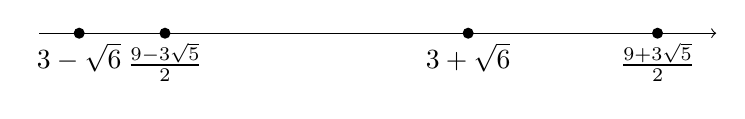
\begin{tikzpicture}
\draw[->] (0,0)--(8.6,0);
\fill (0.51,0) circle [radius=2pt] node [below=0pt] {$3-\sqrt{6}$};

\fill (1.6,0) circle [radius=2pt] node [below=0pt] {$\frac{9-3\sqrt{5}}{2}$};
\fill (5.45,0) circle [radius=2pt] node [below=0pt] {$3+\sqrt{6}$}; 

\fill (7.855,0) circle [radius=2pt] node [below=0pt] {$\frac{9+3\sqrt{5}}{2}$};
\end{tikzpicture}
\end{center}
と並ぶことに注意すると, 次の増減表を得る:
\begin{center}
$
\begin{array}{|c|*5{c|}}\hline
  X & \dfrac{9-3\sqrt{5}}{2} & \cdots  & 3+\sqrt{6} & \cdots  & \dfrac{9+3\sqrt{5}}{2} \\ \hline
  W'(x)&       &  + &   0    & - &      \\ \hline
  W(x) &    & \nea &  \mbox{極大}   &\sea &   \\ \hline
\end{array}
$
\end{center}
よって$V(x)=\dfrac{1}{12}\sqrt{W(X)}$も$X=3+\sqrt{6}$で最大となるので, 
\beqn
&&(V(x)\mbox{の最大値}) \\
&=& \dfrac{1}{12}\sqrt{W(3+\sqrt{6})}\\
&=& \dfrac{1}{12}\sqrt{ -(3+\sqrt{6})\left\{ -(3+\sqrt{6})^{2} + 9(3+\sqrt{6}) - 9 \right\} }\\
&=& \dfrac{1}{12}\sqrt{-(3+\sqrt{6})\left\{3+3\sqrt{6} \right\}}\\
&=& \mbox{   \bolm{     \dfrac{\sqrt{3}}{12}\sqrt{9+4\sqrt{6}}  } }
\eeqn

\subsection{Q.251}
(\textbf{注意}) 図形は, 「1点」と「連結な部分」の和になっている。この図形は楕円曲線と呼ばれる物のひとつであり, 実平面上での一般的な式は
\[y^2 = x^3+ ax + b\quad (a,b\in \mb{R})\]
という方程式である。普通は一つにつながっているか, 閉じた曲線と一つのつながりの和になっているのだが, この閉じた曲線が1点に縮んでいった瞬間の$a,b$を本問で選んできたというわけである。そういうわけで, この1点を非常に見落としやすいというそういう問題である。




\subsection{Q.252}
\subsection*{(1)} $(x,y,z) \neq (0,0,0)$ なる解が存在したとする。$x^2 + y^2\equiv 0\pmod{3}$であるが, 一般に自然数$n$に対して$n^2\equiv 0,1\pmod{3}$であるため, $x,y$はともに$3$の倍数でなければならない。このとき, $3z^2$は$9$の倍数となるから, $z$は$3$の倍数である。すると, この方程式の解に関して
\[(x,y,z) が 整数解 \nara \parena{\frac{x}{3}, \frac{y}{3}, \frac{z}{3}} が整数解\]
が言えるから, この議論を繰り返して$N=0,1,2\cdots$に対して$(\frac{x}{3^{N}}, \frac{y}{3^{N}}, \frac{z}{3^{N}})$ が整数解となる。しかし, $x,y,z$のどれかが$0$ではないから, その$0$でないものに関して, 十分大きい$N$に対してそれを$3^{N}$で割ったものが整数でなくなるから矛盾する。よってこのような解は存在せず, $(x,y,z) = (0,0,0)$は自明な解であるから示された。\qed
\subsection*{(2) (a)} 背理法によって証明する。$\mr{X}$が有理点であるような三角形$\mr{ABC}$が存在したとする。ここで, そのようなものが存在するならば, $\mr{A}$の座標は$(0,0)$であるとしてよい。なぜなら, $\mr{A}$と原点はともに有理点であり, $A$を原点に動かす平行移動によってすべての有理点は有理点へと移動し, $X$の移動先も有理点であるからである。さらに, $\mr{AB}$は有理数であるから, 有理数倍の原点を中心とした拡大縮小によって有理点が有理点に移ることを利用し, $\dfrac{1}{\mr{AB}}$倍によって$\mr{AB}=1$であるとしてもよい。\par
$X$の座標を$(p,q)$とする($p,q$は有理数で)。三角形$\mr{ABC}$の外接円の半径を$R$とすれば, その外接円の方程式は
\[(x-p)^2 + (y-q)^2 = R^2\]
で与えられ これは原点($=\mr{A}$) を通るので$p^2 + q^2 = R^2$が従う。正弦定理によって
\[R = \dfrac{1}{2\sin{\theta}} = \dfrac{1}{\sqrt{3}}\]
であるから, $p^2 + q^2 = \dfrac{1}{3}$である。$p,q$は有理数であったから, $t=p,q$に関して 自然数$x_t$, 整数$y_t$を取って
\[t = \dfrac{y_t}{x_t}\]
と表示することができる。すると, 
\beqn
p^2+q^2 = \dfrac{1}{3} &\iff& \parena{\dfrac{y_p}{x_p}}^2 + \parena{\dfrac{y_q}{x_q}}^2 = \dfrac{1}{3}\\
&\iff& (3y_px_q)^2 + (3y_qx_p)^2 = 3(x_px_q)^2
\eeqn
となり, $x_px_q \neq 0$であるから(1)に反する。よって矛盾であり, $\mr{X}$は有理点でない。\qed
\subsection*{(2) (b)} \tf{存在する。}まず, 不定方程式$x^2 + y^2 = 2020z^2$は非自明な有理数解$(x,y,z) = (12,19,\frac{1}{2})$を持つ\footnote{$(21,8,\frac{1}{2})$でもOK。}ことに注意する。$x_0=12, y_0=19$とおく。\par
$A$を原点とする。$\mr{AB} = 1$となるように作ろう。このとき, 正弦定理より外接円半径は$\sqrt{505}$である。有理点$\mr{X}(p,q)$が取れたとするなら, 外接円の方程式は
\[(x-p)^2 + (y-q)^2 = 505\]
を満たし, それが原点を通るから$p^2 + q^2 = 505$を満たすべきである。そこで, $p,q$として$p=x_0$, $q=y_0$を取ろう。\par
この$\mr{A}(0,0)$と$\mr{X}(x_0,y_0)$から条件を満たすように$\mr{B},\mr{C}$を取ろう。$\mr{B}$の座標を$(a,b)$とする。$\mr{AB}$の垂直二等分線上に外心$\mr{X}$があるように点$\mr{B}$を取るべきであるが, その垂直二等分線の方程式は
\[ax+by = \dfrac{1}{2}\]
である。よって, $a,b$は$a^2 + b^2 = 1$かつ$12a + 19b=\dfrac{1}{2}$を満たすように取ればよく, これを解いて
\[a= \dfrac{6}{505} \pm \dfrac{19\sqrt{2019}}{1010},\quad b=\dfrac{19}{1010}\mp \dfrac{6\sqrt{2019}}{505}\quad (複合同順)\]
を得るので, そのうちの一つとして
\[B = \parena{\dfrac{6}{505} - \dfrac{19\sqrt{2019}}{1010},\dfrac{19}{1010}+ \dfrac{6\sqrt{2019}}{505}}\]
を選ぶ。$\mr{XA} = \mr{XB}$を満たすように取ったから, $(x-x_0)^2 + (y-y_0)^2 = 505$上に$\mr{A},\mr{B}$が存在する。$\mr{C}$は, この円の弧$\mr{AB}$のうち, 長いほうから任意にとればよい。なぜなら, その弧に対する円周角($\angle{\mr{ACB}}$)は鋭角であり, 正弦定理より$\sin{\angle{\mr{ACB}}} = \dfrac{1}{2\sqrt{505}} =\dfrac{1}{\sqrt{2020}}$であるから, $\angle{\mr{ACB}} = \theta$が満たされる。たとえば, $\mr{C}$として$(0,2y_0) = (0,38)$を取る。この点は, $\mr{X}$を通る直線$y=y_0$より上にある。一方で, $\mr{A},\mr{B}$は下にあるので, この$\mr{C}$は弧$\mr{AB}$のうち長いほうに属することも明らかである。以上より, $\mr{A},\mr{B},\mr{C}$の一例として
\[\bolm{\mr{A}(0,0), \mr{B}\parena{\dfrac{6}{505} - \dfrac{19\sqrt{2019}}{1010},\dfrac{19}{1010}+ \dfrac{6\sqrt{2019}}{505}}, \mr{C}(0,38)}\]
を与えることが出来る。
\subsection{余談}
一般化すると次が成り立つ。
\begin{prop}
$0< \theta  \leq \frac{\pi}{2}$を満たす定数$\theta$に対して, 次は同値である。
\ben
\item (\tf{条件})を満たす三角形$\mr{ABC}$が存在する。
\item $\sin{\theta}$は有理数である。または, $4k+3$型素数の約数と平方因子を持たない自然数$n$と, (正の)有理数$r$を用いて$\sin{\theta} = r\sqrt{n}$と表すことが出来る。
\een
\end{prop}
この証明のためには, (2)の条件にあるような$n$に関して$x^2 + y^2 = nz^2$が非自明な整数解を持ち, 逆に平方因子を含まず$4k+3$型素数の約数を持てば非自明な整数解を持たないことを示す必要があり, それは「二平方和定理」より従う。このことを事実として認めれば, (2) (a)と同じ方法によって, (1)$\nara (2)$が従う。(2)$\nara$(1)は(2) (b)と同じような構成で分かる。また, $\theta$を鈍角にしてもよい($\mr{C}$を取るときに短い方の弧$\mr{AB}$から取ればよい)。




\clearpage
\section{2/9}
\subsection{Q.247}
あえて答えがいくつかに分かれそうな書き方をした。自由に論じてもらえば良いが, もっともらしいことを言わなければならない。\par
$f\in \mb{R}[x]\setminus{\{ 0 \}}$に対して, その次数を$\deg{f}$と書くことにしよう。このとき, 次が成り立つことは明らかである。
\[\deg{(fg)} = \deg{f} + \deg{g}\quad (f,g\in \mb{R}[x]\setminus{\{ 0 \}})\]
仮に$\deg{0}$を定義しようものなら, この公式を$f=0, g=0$の場合にも拡張したいと考えたくなるものである。では形式的に$g=0$としてみると
\[\deg{0} = \deg{f} + \deg{0}\]
となり, $\deg{0}$は普通の実数のような数では定義しづらい。そこで, 極限計算的には正しい$\infty + x = \infty$, $-\infty + x = -\infty$のような式を思い出し, $\deg{0} = \infty$または$\deg{0} = -\infty$とするとこの公式は「ある意味では崩れない」感じがする。\par 
さて, 現段階では$\pm \infty$のどちらも妥当である。そこで, 他に$\deg{f}$にまつわる公式がないかを探し, その公式を$\deg{0}$が入る場合に拡張出来ないかということを再び考えてみよう。たとえば次のようなものがある。
\[\deg{(f+g)} \leq  \max{\{ \deg{f}, \deg{g}\} } \quad (f,g,f+g\neq 0)\]
形式的に$f+g = 0$であるとすると
\[\deg{0} \leq \max{\{ \deg{f}, \deg{(-f)}\} } = \deg{f}\]
となる。この式を見るに, $\deg{0} = \infty$とはしづらい。$\infty \leq \deg{f}$は奇妙だからである。一方で$\deg{0} = -\infty$はこの点に関しては問題がない!\par 
その他, $\deg{0} = -\infty$とするのが有用そうであると思える点はある。たとえば, 
\ben 
\item 剰余の定理を思いだそう。$g(x)\neq 0$とする。$f$の$g$による割り算を実行した$f(x) = g(x)Q(x) + R(x)$ ($Q(x)$は整式, $R(x) = 0$または$R\neq 0$かつ$\deg{R} < \deg{g}$) における$R$の条件は, $\deg{0} = -\infty$, $-\infty < r$ ($r\in \mb{R}$)と取り決めるならば「$\deg{R} < \deg{g}$」とだけ書いてもよいだろう。 
\een

$\deg{0} = \infty$としたい理由もいくつか考えられる。
\ben
\item $f\neq 0$のとき, $\deg{f}$は方程式$f(x) = 0$の複素数解の個数である。だから$\deg{0} = \infty$が相応しい。
\item ・・・
\een
個人的には, これを理由にするのはいささか微妙なのではと思う。確かに(1)のような事実はある。しかしながらそれは$\deg{f}$の「生の情報」と言えるかどうかは少し怪しい。つまり, 多項式の零点の個数は$\deg{f}$と同じだという事実が先走り, それが$\deg{f}$の本質だ, と主張できるかどうかは微妙ではないかと思うのである。まるで「1ってなんですか?」という哲学的な問いに対して「乗法単位元です」と答えているかのようだ\footnote{実際に見たことがある。}。多項式は関数とも見れるが, 関数と思わない視点もある。$\deg{f}$は多項式を関数と思わずとも定まる概念である。だから, 零点の個数(関数の視点による情報)はやや$\deg{f}$の概念から離れているのではないかと思う。\par
結局, 「$\deg{}$というのは$\mb{R}[x]\setminus{\{ 0 \}}$に対して整数値を与える写像にすぎない」という立場からすれば, 零点の個数と話を結びつけるのは自然とは言いがたい。一方で$\deg{0} = -\infty$を採用するに至った方法では, $\deg{}$という写像に関する話の範囲内である。だから, より生の$\deg{}$を使って話が展開できているのではないだろうか。

\subsection{Q.173}
$n! - 1$は$2$以上$n$以下の自然数$k$で割ると必ず$k-1$だけ余るので, $n!-1$は$k$の倍数ではない。つまり, $n!-1$の1より大きい約数は必ず$n$より大きい。$n\geq 3$より$n!-1>1$であるから, $n!-1$はある素数$p$で割り切れるが, そのような$p$がまさしく$n < p < n!$を満たす素数である。\qed
\end{document}
